%\documentclass[11pt,a4paper,titlepage,twoside]{article}
\documentclass[12pt,a4paper,twoside]{article}
%\documentclass[12pt,a4paper,twoside]{scrartcl}
\usepackage{mystyle}
\usepackage{gplot}
\usepackage{mechanik_v001}


%\author{Felix Binder}
\title{Mechanik}
\date{}



\def\dir{./Aufgaben_Mechanik/}
\newcommand{\Einbinden}[1]{\input{#1}}


\begin{document}
\maketitle

%\startkloesung

\section{Grössen und Einheiten}
\subsection{Weg}

Eine sehr wichtige Grösse in der gesamten Physik ist der Weg. 
Um die Länge eines Weges zu bestimmen muss man ihn messen.
Messen bedeutet vergleichen mit einer Einheit.
Das Formelzeichen für den Weg ist $s$. 
Die Grundeinheit (SI-Einheit, von französisch Système international d’unités) des Weges ist der Meter.
Abgekürzt wird die Einheit mit \si{m}.
Die Einheit einer physikalischen Grösse schreibt man in eckigen Klammern, also $[s]=\si{m}$.

\Einbinden{\dir/einheiten01.tex}
\Einbinden{\dir/einheiten02.tex}
\Einbinden{\dir/einheiten03.tex}
\Einbinden{\dir/einheiten04.tex}

\subsection{Zeit}
Um die Zeit $t$ zu messen, orientiert sich die Menschheit schon seit Jahrtausenden an den Gestirnen.
Winter- und Sommersonnenwenden wurden schon in der Steinzeit gefeiert.
Das Messgerät zur Zeitmessung ist die Uhr.
Die SI-Einheit der Zeit ist die Sekunde (s).
Traditionell ist die Sekunde der \num{86400}-ste Teil $(24\cdot60\cdot60)$ eines Tages.
Seit 1967 wird die Sekunde über eine atomare Anregung definiert. Daher auch der Name Atomuhr.

\Einbinden{\dir/einheiten05.tex}

\subsection{Masse}
Eine weitere häufig gebrauchte Grösse ist die Masse $m$. Ihre SI-Einheit ist das Kilogramm (kg).
Anders als bei den anderen Einheiten, hat das Kilogramm noch keine moderne, ausschliesslich auf
Naturkonstanten basierende Definition. Das Urkilogramm besteht aus einer Platin-Iridium-Legierung und wird in Paris verwahrt.


\Einbinden{\dir/einheiten06.tex}
\Einbinden{\dir/einheiten07.tex}
\Einbinden{\dir/einheiten08.tex}





\newpage

\section{Kinematik}



\Einbinden{\dir/geschwindigkeit00a.tex}
\Einbinden{\dir/geschwindigkeit00b.tex}

\Einbinden{\dir/geschwindigkeit01.tex}
\Einbinden{\dir/geschwindigkeit02.tex}
\Einbinden{\dir/geschwindigkeit03.tex}
\Einbinden{\dir/geschwindigkeit04.tex}
\newpage
\Einbinden{\dir/geschwindigkeit05.tex}

\newpage
\Einbinden{\dir/geschwindigkeit06.tex}
\Einbinden{\dir/geschwindigkeit07.tex}

\newpage

\Einbinden{\dir/beschleunigung01.tex}
\Einbinden{\dir/beschleunigung02.tex}
\Einbinden{\dir/kinematik01.tex}

\newpage
\newpage
\begin{aufgabe}
	\label{ExpWasserstrahl}
	Sie sehen ein Experiment mit einem Wasserstrahl.
	\begin{enumerate} [a)]
		\item	Schreiben Sie sich Fragen auf, die Ihnen zu diesem Experiment einfallen.
		\item	Diskutieren Sie Ihre Fragen mit Ihrem Nachbarn und versuchen Sie Antworten auf Ihre Fragen zu finden.
	\end{enumerate}

	\textbf{Tipp:} Es ist immer gut eine Skizze des Experiments anzufertigen.

\end{aufgabe}

\begin{aufgabe}
Ein Tropfen Wasser fällt aus einer Höhe von 50 Zentimeter zu Boden.
Wie lange braucht der Wassertropfen um die Erde zu erreichen?
\kloesung{\SI{0.32}{s}}
\end{aufgabe}

\begin{aufgabe}
Nehmen Sie an, Sie leben in einer Welt ohne Schwerkraft.
Was müssten Sie bei einer Wasserschlacht mit Wasserpistolen beachten?
\end{aufgabe}

\begin{aufgabe}
	Nehmen Sie an, ein Tropfen eines Wasserstrahls kommt mit einer Geschwindigkeit von \SI{2}{m/s}
	parallel zum Boden aus einem Schlauch.

	Welche Strecke $s_x$ legt der Tropfen in horizontaler Richtung zurück?
	Welche Strecke $s_y$ legt der Tropfen in Richtung des Bodens zurück?

	\begin{enumerate} [a)]
		\item	Füllen Sie die Tabelle:

	\begin{tabular}{p{4cm}|p{4cm}|p{4cm}}
			$\Delta t$ (s) & $s_x$ (m) & $s_y$ (m)\\\hline
			\num{0.1} & & \\
			\num{0.2} & & \\
			\num{0.3} & & \\
			\num{0.4} & & \\
			\num{0.5} & & \\
		\end{tabular}

	\item Zeichen Sie den Wasserstrahl mit Hilfe der berechneten Werte.
	
	\end{enumerate}
\end{aufgabe}

\newpage

\begin{aufgabe}
	In Aufgabe \ref{ExpWasserstrahl} haben Sie einen Experiment mit einem Wasserstrahl gesehen.
	Beantworten Sie zu diesem Experiment folgende Fragen:
	\begin{enumerate}[a)]
		\item	Wie lange fällt ein Wassertropfen des Wasserstrahls bis dieser den Boden erreicht.
		\item	Wie hoch ist die Geschwindigkeit des Wasserstrahls beim Austritt aus der Flasche.
	\end{enumerate}
\end{aufgabe}


\Einbinden{\dir/beschleunigung03.tex}
\Einbinden{\dir/bew3d01.tex}

\newpage
\section{Kräfte}
\Einbinden{\dir/vektoren01.tex}
\Einbinden{\dir/vektoren02.tex}
\Einbinden{\dir/vektoren03.tex}
\Einbinden{\dir/vektoren04.tex}


\newpage

\begin{aufgabe}
	Messen Sie in kleinen Gruppen (etwa vier Personen)
	wie ein Spielzeugauto durch das Anhängen eines Gewichtes beschleunigt wird.

	Befestigen Sie dazu einen Faden am Auto. Am anderen Ende des Fadens befestigen Sie
	Gewichte, die Sie dann über die Tischkante rutschen lassen.

	Tragen Sie die Messwerte in die Tabelle ein. 
	Berechnen Sie die Gewichtskraft, die das Auto antreibt und die Beschleunigung des Autos.
	Messen Sie auch das Gewicht des Autos.

	Tragen Sie Kraft und Beschleunigung in ein Koordinatensystem ein ($x$-Achse Beschleunigung, $y$-Achse Kraft).

\newcommand\leereZ{\phantom{x} & & & &  \\\hline}


	\begin{center}
		
		\begin{tabular}{p{0.15\textwidth}|p{0.15\textwidth}|p{0.15\textwidth}||p{0.15\textwidth}|p{0.15\textwidth}}
			\multicolumn{3}{c||}{Messwerte} & \multicolumn{2}{c}{Berechnete Grössen}\\
			$\Delta s$ (m) & $\Delta t$ (s) & $m$ (kg) & $a$ (m/s$^2$)& $F$ (N)\\\hline
			
\leereZ
\leereZ
\leereZ
\leereZ
\leereZ
\leereZ
		\end{tabular}

		\Karo{9.5}
	
	\end{center}

\end{aufgabe}



%\section{Die Dichte}

\begin{table}
	\centering
	\begin{tabular}{c r | c r | c r}
		Gold                             & 19290  & 	Sandstein     & 2400 & Ethanol  & 789\\
		Quecksilber                      & 13546  & 	Glas          &2500  & Diesel   & 830\\
		Aluminium                        &  2700  & 	Diamant       & 3510 & Olivenöl & 910\\
		Wasser (\SI{0}{\degreeCelsius})  &  1000  & 	Silber        & 10490& Meerwasser& 1025 \\
        Eis (\SI{0}{\degreeCelsius})     &   917  & 	Uran          & 19050& Milch    & 1030\\
		Holz (Kiefer)                    &   520  & 	Platin        & 21450& Helium (\SI{0}{\degreeCelsius})   & \num{0,1785}\\
		Luft                             &  1.2041& 	Blei          & 11340& Wasserstoff (\SI{0}{\degreeCelsius}) & \num{0,0899}\\
	\end{tabular}
	\caption{Dichte verschiedener Materialien in (\si{kg}/\si{m}$^3$).}
	\label{tab:dichte}
\end{table}


Die Dichte ($\rho$) ist das Verhältnis zwischen Masse (m) und Volumen (V).


\begin{cbox}
\begin{equation*}
	\rho = \frac{\text{Masse}}{\text{Volumen}} = \frac{m}{V}\text{,}\quad\text{Einheit:} [\rho]=\frac{\text{kg}}{\text{m}^3} 
\end{equation*}
\end{cbox}

Die Dichte ist eine Materialkonstante und kann zur Unterscheidung verschiedener Materialien
verwendet werden. Sie ist unabhängig von Form und Grösse des Gegenstands. 
Die Dichte von Festkörpern ist grösser als die Dichte von Gasen.
In Tabelle \ref{tab:dichte} sind die Dichten einiger Materialien angegeben.

\Einbinden{\dir/dichte01.tex}
\Einbinden{\dir/dichte02.tex}
\Einbinden{\dir/dichte03.tex}
\Einbinden{\dir/dichte04.tex}


%\section*{Weg}
%\input{./Abbildungen/weg.tex}
%\newpage
%\section{Geschwindigkeit}
Die Geschwindigkeit ist eine abgeleitete Grösse. Sie gibt an, wie viel Weg $\Delta s$ in einem Zeitintervall $\Delta t$
zurückgelegt werden.
Wenn sich weder Betrag noch Richtung der Geschwindigkeit ändern, so spricht man von einer \emph{gradlinig gleichförmig} Geschwindigkeit. 
\begin{cbox}
\begin{gather*}
	\text{Geschwindigkeit} = \frac{\text{Weg}}{\text{Zeit}}\quad\text{oder}\quad \bar{v}=\frac{\Delta s}{\Delta t}\\
		\text{Einheit}: [v] = \frac{\text{Meter}}{\text{Sekunde}}=\frac{\si{m}}{\si{s}}
\end{gather*}
\end{cbox}

Mit dem Strich über dem $\bar{v}$ wird angedeutet, dass eine durchschnittliche Geschwindigkeit
gemeint ist. Diese kann von der \emph{Momentangeschwindigkeit} abweichen, wenn das bewegte Teilchen beschleunigt wird.

\Einbinden{\dir/geschwindigkeit01.tex}
\Einbinden{\dir/geschwindigkeit02.tex}
\Einbinden{\dir/geschwindigkeit03.tex}
\Einbinden{\dir/geschwindigkeit04.tex}
\Einbinden{\dir/geschwindigkeit05.tex}


%\newpage
%\section*{Beschleunigung}
Die Beschleunigung ist eine abgeleitete Grösse. Sie gibt an, wie sich die Geschwindigkeit
mit der Zeit ändert.

Die Bewegung eines Massenpunktes heisst \emph{gradlinig gleichförmig beschleunigt}, wenn der Körper sich
mit einer konstanten Beschleunigung $a$ geradlinig bewegt.
Wird er konstant beschleunigt, ändert sich seine Geschwindigkeit linear mit der Zeit.

\begin{cbox}
\begin{gather*}
	\text{Beschleunigung} = \frac{\text{Geschwindigkeit}}{\text{Zeit}}\quad\text{oder}\quad \bar{a}=\frac{\Delta v}{\Delta t}\\
		\text{Einheit}: [a] = \frac{\text{Meter}}{\text{Sekundequadrat}}=\frac{\si{m}}{\si{s^2}}
\end{gather*}
\end{cbox}

Mit dem Strich über dem $\bar{a}$ wird angedeutet, dass eine durchschnittliche Beschleunigung 
gemeint ist.

\Einbinden{\dir/beschleunigung01.tex}
\Einbinden{\dir/beschleunigung02.tex}




\section*{Bewegungsdiagramme}
Zeitliche Bewegungsabläufe können übersichtlich in Bewegungsdiagrammen dargestellt werden.
Dabei werden die physikalischen Grössen Weg ($s$), Geschwindigkeit ($v$) und Beschleunigung ($a$) als Funktion
der Zeit dargestellt.


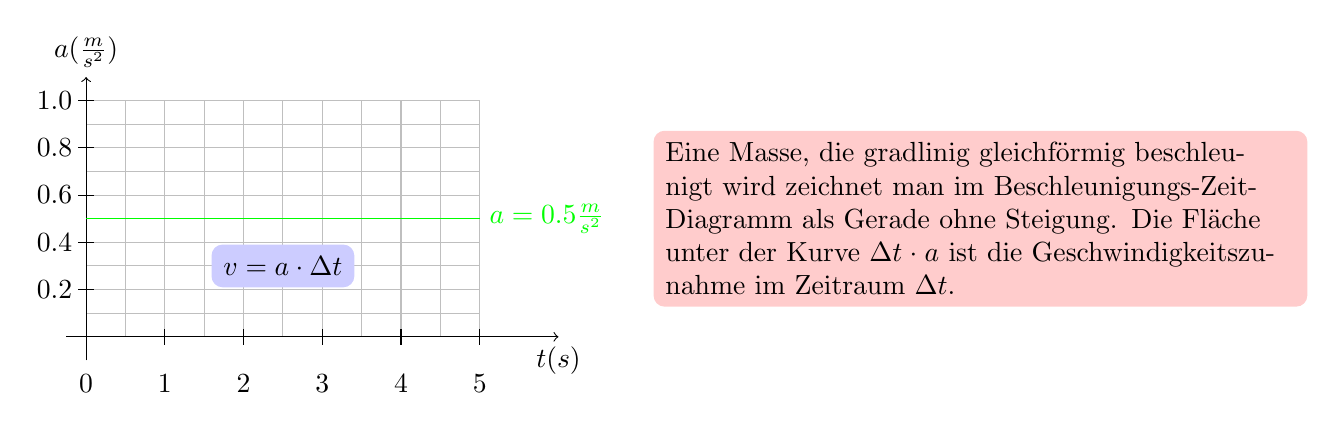
\begin{tikzpicture}[scale=1,yscale=3, info box/.style={rounded corners, inner sep=1ex}, info text/.style={info box, fill=red!20}]
\usetikzlibrary{calc,intersections,through,backgrounds}
\draw[step=0.5cm,ystep=0.1,lightgray] (0,0) grid (5.0,1.0);

%begin Koordinatensystem
%x-achse
\coordinate (C1) at (-0.25,0);
\coordinate [label=below:$t (s)$] (C2) at (6,0);
\draw  [->] (C1)--(C2);
\foreach \x in {0,1,2,3,4,5}
{
\draw (\x,-0.2) node {\x};
\draw (\x,-0.1/3)--(\x,0.1/3);
}


%y-achse
\coordinate (C3) at (0,-0.1);
\coordinate [label=above:$a (\frac{m}{s^2})$] (C4) at (0,1.1);
\draw [->] (C3)--(C4);
\foreach \y in {0.2,0.4,0.6,0.8,1.0}
{
\draw (-0.4,\y) node {\y};
\draw (-0.1,\y)--(0.1,\y);
}
%end Koordinatensystem

\draw  [color=green,domain=0:5] plot (\x,0.5) node [above,right] {$a=\SI{0.5}{\frac{m}{s^2}}$};
\draw (2.5,0.3) node [info box, fill = blue!20] {$v=a\cdot \Delta t$};

%infokasten
\draw [xshift=7.2cm] (0,0.5) node [right, text width=8cm, info text] {
Eine Masse, die  gradlinig gleichförmig beschleunigt wird zeichnet man
im Beschleunigungs-Zeit-Diagramm als Gerade ohne Steigung.
Die Fläche unter der Kurve $\Delta t\cdot a$ ist die Geschwindigkeitszunahme im Zeitraum $\Delta t$.
};



\end{tikzpicture} 


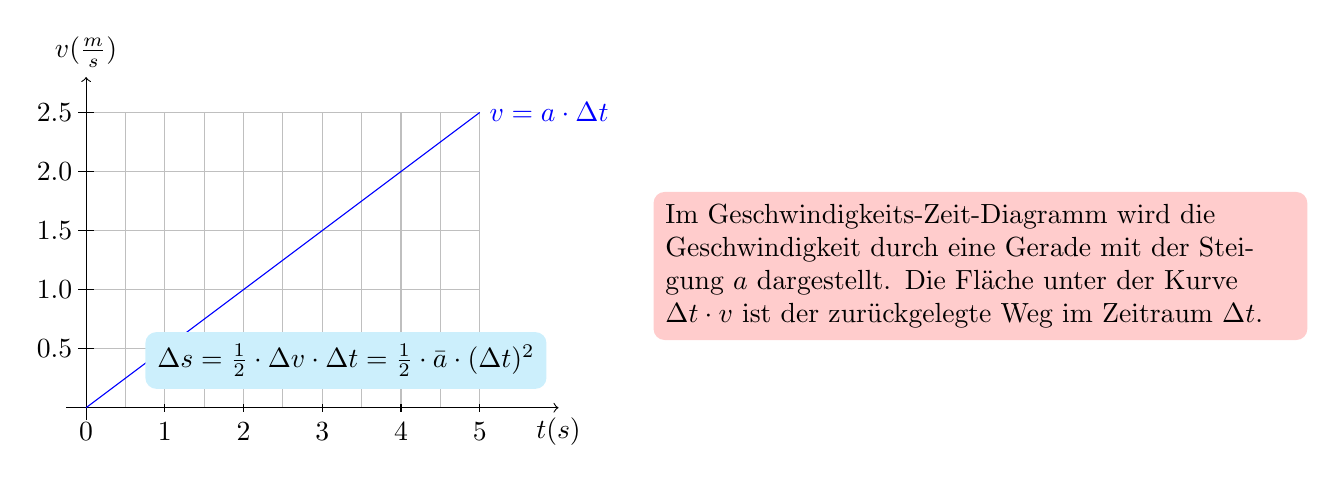
\begin{tikzpicture}[scale=1,yscale=1.5, info box/.style={rounded corners, inner sep=1ex}, info text/.style={info box, fill=red!20}]
%\usetikzlibrary{calc,intersections,through,backgrounds}
\draw[step=0.5cm,ystep=0.5,lightgray] (0,0) grid (5.0,2.5);

%begin Koordinatensystem
%x-achse
\coordinate (C1) at (-0.25,0);
\coordinate [label=below:$t (s)$] (C2) at (6,0);
\draw  [->] (C1)--(C2);
\foreach \x in {0,1,2,3,4,5}
{
\draw (\x,-0.2) node {\x};
\draw (\x,-0.1/3)--(\x,0.1/3);
}


%y-achse
\coordinate (C3) at (0,-0.1);
\coordinate [label=above:$v (\frac{m}{s})$] (C4) at (0,2.8);
\draw [->] (C3)--(C4);
\foreach \y in {0.5,1.0,1.5,2.0,2.5}
{
\draw (-0.4,\y) node {\y};
\draw (-0.1,\y)--(0.1,\y);
}
%end Koordinatensystem

\draw  [color=blue,domain=0:5] plot (\x,0.5*\x) node [above,right] {$v=a\cdot\Delta t$};
\draw (3.3,0.4) node [info box, fill =cyan!20] {$\Delta s=\frac{1}{2}\cdot \Delta v\cdot \Delta t = \frac{1}{2}\cdot\bar{a}\cdot(\Delta t)^2$};

%infokasten
\draw [xshift=7.2cm] (0,1.2) node [right, text width=8cm, info text] {
Im Geschwindigkeits-Zeit-Diagramm wird die Geschwindigkeit durch eine Gerade
mit der Steigung $a$ dargestellt. 
Die Fläche unter der Kurve $\Delta t\cdot v$ ist der zurückgelegte Weg im Zeitraum $\Delta t$.
};



\end{tikzpicture} 


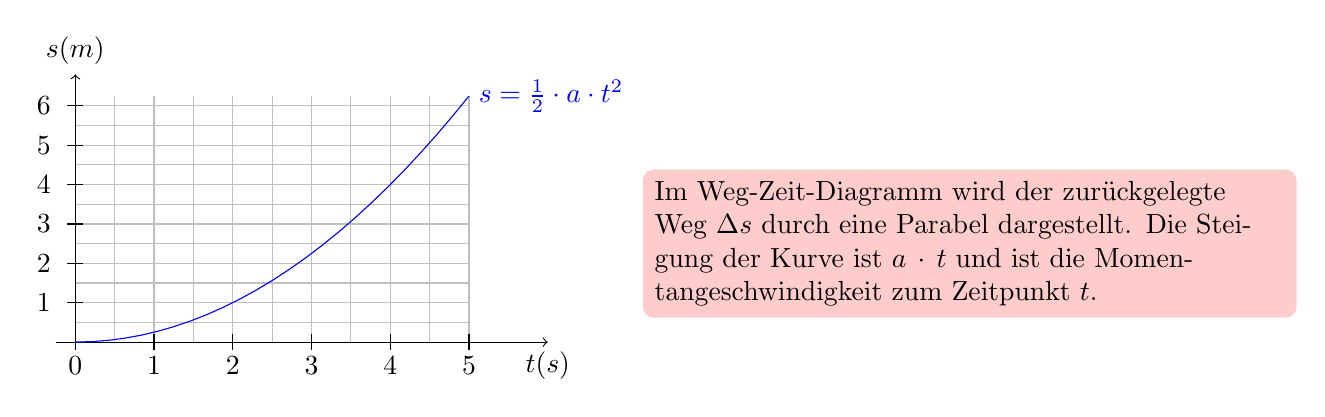
\begin{tikzpicture}[scale=1,yscale=0.5, info box/.style={rounded corners, inner sep=1ex}, info text/.style={info box, fill=red!20}]
%\usetikzlibrary{calc,intersections,through,backgrounds}
\draw[step=0.5cm,ystep=0.5,lightgray] (0,0) grid (5.0,6.25);

%begin Koordinatensystem
%x-achse
\coordinate (C1) at (-0.25,0);
\coordinate [label=below:$t (s)$] (C2) at (6,0);
\draw  [->] (C1)--(C2);
\foreach \x in {0,1,2,3,4,5}
{
\draw (\x,-0.6) node {\x};
\draw (\x,-0.1/0.5)--(\x,0.1/0.5);
}


%y-achse
\coordinate (C3) at (0,-0.1);
\coordinate [label=above:$s (m)$] (C4) at (0,6.8);
\draw [->] (C3)--(C4);
\foreach \y in {1,2,3,4,5,6}
{
\draw (-0.4,\y) node {\y};
\draw (-0.1,\y)--(0.1,\y);
}
%end Koordinatensystem

\draw  [color=blue,domain=0:5] plot (\x,0.25*\x*\x) node [above,right] {$s=\frac{1}{2}\cdot a\cdot t^2$};
%\draw (3.3,0.4) node [info box, fill =cyan!20] {$\Delta s=\frac{1}{2}\cdot \Delta v\cdot \Delta t = \frac{1}{2}\cdot\bar{a}\cdot(\Delta t)^2$};

%infokasten
\draw [xshift=7.2cm] (0,2.5) node [right, text width=8cm, info text] {
Im Weg-Zeit-Diagramm wird der zurückgelegte Weg $\Delta s$ durch eine Parabel dargestellt. 
Die Steigung der Kurve ist $a\cdot t$ und ist die Momentangeschwindigkeit zum Zeitpunkt $t$.
};



\end{tikzpicture} 




Aus den Bewegungsdiagrammen lassen sich zwei wichtige Formeln ablesen.
%\begin{cbox}
\begin{equation*}
	v=v_0+a\cdot t \qquad s=s_0 + v_0\cdot t+\frac{1}{2}\cdot a\cdot t^2
\end{equation*}
%\end{cbox}
Durch auflösen der ersten Gleichung $v=v_0+a\cdot t$ nach t und einsetzen in die zweite
bekommen wir eine Gleichung, in der die Zeit $t$ nicht vorkommt.
\begin{equation*}
	v^2=v_0^2+2\cdot a\cdot (s-s_0)
\end{equation*}

\Einbinden{\dir/beschleunigung02.tex}



%\section*{Der freie Fall}

Eine Masse fällt im Schwerefeld der Erde runter. Wie läuft der Fall der Masse ab?
Diese Frage kann mit dem Aufbau eines Experimentes beantwortet werden.
Dazu lassen wir eine Metallkugel aus einer vorher festgelegten Höhe zu Boden fallen.
Die Kugel benötigt für den Fall eine bestimmte Zeit $\Delta t$ die wir messen.
Um Fehler durch die Messung zu verringern, nehmen wir mehrere Zeitmessungen zu jeder
Höhenänderung vor und mitteln die Zeitspanne.
Dies wird für verschiedene Fallhöhen wiederholt. 
Die ermittelten Zeiten werden in einem Weg-Zeit-Diagramm eingetragen.


\begin{minipage}{0.5\textwidth}
%\begin{table}
	\centering
	\begin{tabular}{ccc}
		$\Delta s (\si{m})$ & $\Delta t (\si{ms})$ & $\overline{\Delta t} (\si{ms})$ \\\hline
0.1 & 129 131 130 & 130\\
0.2 & 195 200 201 & 199\\
0.3 & 241 248 244 & 244\\
0.4 & 278 285 276 & 280\\
	\end{tabular}
%	\caption{Messprotokoll für den freien Fall einer Metallkugel.}
%	\label{tab:freierfall1}
%\end{table}
\end{minipage}
\begin{minipage}{0.5\textwidth}
	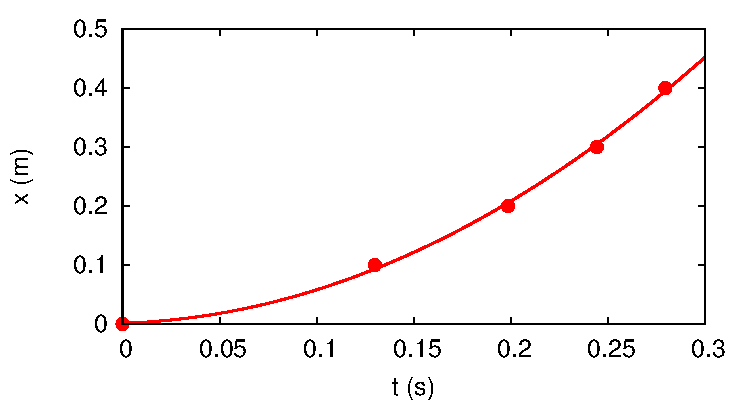
\includegraphics[width=0.95\textwidth]{./freierfall_xt.pdf}
\end{minipage}

Nun wollen wir aus dem Weg-Zeit-Diagramm ein Geschwindigkeits-Zeit-Diagramm erstellen.
Dabei gibt es einige Schwierigkeiten. Für das $v$-$t$-Diagramm wird die Momentangeschwindigkeit
benötigt. Durch die Messung kann allerdings nur eine mittlere Geschwindigkeit bestimmt werden.
Damit die mittlere Geschwindigkeit möglichst nahe an der Momentangeschwindigkeit ist, sollte eine
möglichst kleine Zeitspanne $\Delta t$ betrachtet werden.
Wir berechnen die Geschwindigkeit für die jeweils letzten \SI{10}{cm}.



\begin{minipage}{0.5\textwidth}
%\begin{table}
	\centering
	\begin{tabular}{ccc}
	$\Delta s$ &	$\Delta t (\si{s})$ & $\bar{v} (\si{m/s})$ \\\hline
%Geschwindigkeits-Zeit-Tabelle
%die letzten 10 cm
0   & 0         & 0 \\
0.1 & $\SI{130}{ms} -\SI{0}{ms}=\SI{130}{ms}$  & 0.77 \\ 
0.2 & $\SI{199}{ms} -\SI{130}{ms}=\SI{69}{ms}$  & 1.45 \\ 
0.2 & $\SI{244}{ms} -\SI{199}{ms}=\SI{45}{ms}$  & 2.22 \\ 
0.2 & $\SI{280}{ms} -\SI{244}{ms}=\SI{36}{ms}$  & 2.78 \\ 
	\end{tabular}
%	\caption{Messprotokoll für den freien Fall einer Metallkugel.}
%	\label{tab:freierfall1}
%\end{table}
\end{minipage}
\begin{minipage}{0.5\textwidth}
	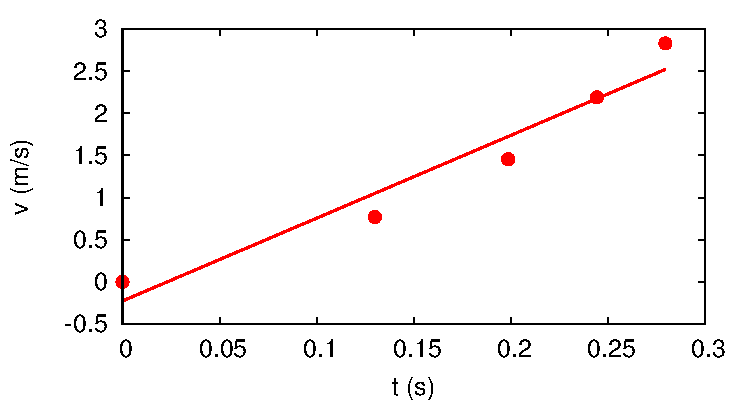
\includegraphics[width=0.95\textwidth]{./freierfall_vt.pdf}
\end{minipage}

Die berechneten Durchschnittsgeschwindigkeiten benutzen wir nun als Momentangeschwindigkeiten und tragen 
die Werte im $v$-$t$-Diagramm ein. Die Steigung der Geschwindigkeitskurve im $v$-$t$-Diagramm ist
\SI{9.92}{m/s^2}. Damit haben wir mit relativ einfachen Mitteln den Wert für die Fallbeschleunigung 
auf der Erde reproduziert und gezeigt, dass ein fallendes Objekt gleichmässig gleichförmig beschleunigt
wird, wenn es sich im Schwerefeld der Erde befindet.
Mit diesem Wissen ist es nicht mehr nötig die Momentangeschwindigkeit durch eine Durchschnittsgeschwindigkeit
zu approximieren. Stattdessen kann die Fallbeschleunigung aus dem Weg-Zeit-Diagramm bestimmt werden. 
Die Geschwindigkeit berechnet sich dann mit $v=g\cdot t$.

%\section*{Bewegung in drei Raumrichtungen}

\subsection*{Vektoren}
Physikalische Grössen wie die Geschwindigkeit $v$, die Beschleunigung $a$ oder auch der Weg $s$ sind
vektorielle Grössen. Ein Vektor hat nicht nur eine Grösse, sondern auch noch eine Richtung.
Vektoren werden daher oft als Pfeile gezeichnet. Die Länge des Pfeils ist dann der Betrag des Vektors,
die Richtung des Pfeils gibt die Richtung des Vektors an.

Ein Vektor kann mit einem geeigneten Koordinatensystem in Komponenten zerlegt werden.


Vektoren kann man graphisch addieren.

%
\section*{Addition von Kräften}

In einem Knoten laufen drei Fäden zusammen. An dem jeweils anderen Ende der Fäden ist eine Masse angehängt.
Zwei der drei Fäden werden durch Rollen umgelenkt.
Wird der Knoten aus seiner Ruhelage (Gleichgewichtslage) ausgelenkt, so pendelt sich das System wieder in diese Lage zurück.
Die Rollen lenken die Fadenkräfte um, ändern aber nicht ihren Betrag.
In der Ruhelage ist die Summe aller angreifenden Kräfte Null.

\Einbinden{\dir/vektoren01.tex}
\Einbinden{\dir/vektoren02.tex}
\Einbinden{\dir/vektoren03.tex}
\Einbinden{\dir/vektoren04.tex}


\newpage
\section*{Zerlegung von Kräften}

Vektoren lassen sich nicht nur addieren, sondern man kann sie auch in Komponenten zerlegen. Das ist im Prinzip die Umkehrung
der Vektoraddition.

\Einbinden{\dir/vektoren05.tex}
\Einbinden{\dir/vektoren06.tex}


Ist die Richtung eines Vektors vorgegeben, lässt sich der Vektor noch nicht eindeutig zerlegen. Es gibt immer
noch viele verschiedene Möglichkeiten den Vektor zu zerlegen.

\newpage


Sind die Richtungen von zwei Vektoren gegeben (in 2D), ist die Zerlegung eindeutig möglich. Allgemein gilt, dass man
für jede Raumdimension eine eindeutige Richtung benötigt.

\Einbinden{\dir/vektoren07.tex}


In der Praxis zerlegt man Vektoren oft in Kartesische Koordinaten, also in eine $x$-, eine $y$- und im Fall von drei Dimensionen in eine $z$-Koordinate.

\Einbinden{\dir/vektoren08.tex}

\newpage

\Einbinden{\dir/vektoren09.tex}

\newpage
\Einbinden{\dir/vektoren10.tex}

\Einbinden{\dir/vektoren11.tex}


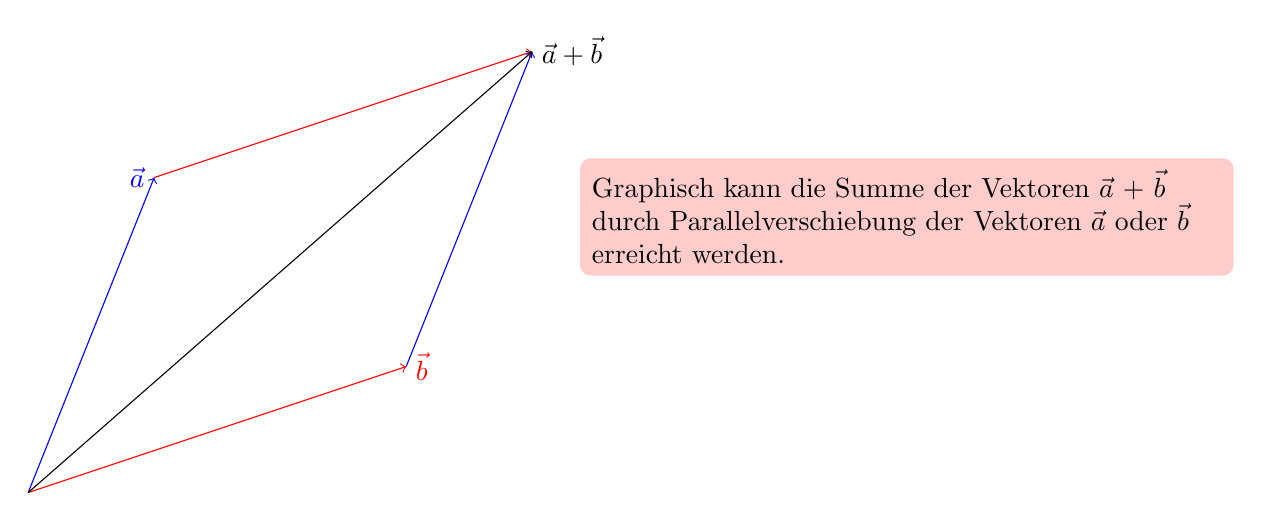
\begin{tikzpicture}[info text/.style={rounded corners, fill=red!20, inner sep=1ex}]
%\begin{tikzpicture}
%\usetikzlibrary{calc,intersections,through,backgrounds}
%\usetikzlibrary{decorations.pathmorphing}
%\draw[step=0.5cm,lightgray] (-0.5,-3.0) grid (6.5,5.0);


\draw [->, blue,scale=0.8] (0,0)--(2,5) node [left] {$\vec{a}$};
\draw[->,red,scale=0.8] (2,5)--+(6,2);

\draw[->,red,scale=0.8] (0,0)--(6,2) node [right] {$\vec{b}$};

\draw[->,blue,scale=0.8] (6,2)--+(2,5);


\draw[->,black,scale=0.8](0,0)--(8,7) node [right]{$\vec{a}+\vec{b}$};
%infokasten
\draw [xshift=7.0cm] (0,3.5) node [right, text width=8cm, info text] {
Graphisch kann die Summe der Vektoren $\vec{a}+\vec{b}$ durch Parallelverschiebung
der Vektoren $\vec{a}$ oder $\vec{b}$ erreicht werden.
};

\end{tikzpicture}

Das bedeutet, dass man eine komplizierte Bewegung, wie zum Beispiel die Bewegung eines geworfenen
Balls, oder einer Pistolenkugel für jede Raumrichtung unabhängig voneinander lösen kann.
Dies macht es erst möglich Bewegungsabläufe in mehr als einer Dimension zu berechnen.

\Einbinden{\dir/bew3d01.tex}
\Einbinden{\dir/bew3d02.tex}





%\newpage
%\printkloesung

\newpage
\includesolutions

\end{document}
